\documentclass[../main.tex]{subfiles}
\begin{document}

\chapter{Cơ sở lý thuyết}

\section{Mô hình toán học}
    
Bài toán đặt ra khi ta cần vận chuyển một loại hàng hóa thuần nhất từ $m$ trạm phát đến $n$ trạm thu, trong đó:
\begin{itemize}
    \item Trữ lượng hàng hóa tại các trạm phát $i \in I = \{1, 2, \dots, m\}$ lần lượt là $a_1, a_2, \dots, a_m$.
    \item Nhu cầu hàng hóa tại các trạm thu $j \in J = \{1, 2, \dots, n\}$ lần lượt là $b_1, b_2, \dots, b_n$.
    \item Cước phí để vận chuyển một đơn vị hàng hóa từ trạm phát $i$ đến trạm thu $j$ là $c_{ij}$.
\end{itemize}

Gọi $x_{ij}$ là lượng hàng hóa được vận chuyển từ trạm phát $i$ đến trạm thu $j$. Khi đó, bài toán vận tải được mô hình hóa dưới dạng một bài toán Quy hoạch tuyến tính (QHTT) như sau \cite{hitchcock1941, kantorovich1939, koopmans1949}:
    
\begin{equation} \label{eq:objective}
    \min f(X) = \sum_{i=1}^{m} \sum_{j=1}^{n} c_{ij} x_{ij}
\end{equation}
với các điều kiện ràng buộc:
\begin{align}
    \sum_{j=1}^{n} x_{ij} &= a_i, \quad \forall i = \overline{1,m} \label{eq:supply} \\
    \sum_{i=1}^{m} x_{ij} &= b_j, \quad \forall j = \overline{1,n} \label{eq:demand} \\
    x_{ij} &\ge 0, \quad \forall i = \overline{1,m}, \forall j = \overline{1,n} \label{eq:nonnegative}
\end{align}
Hệ ràng buộc \eqref{eq:supply} đảm bảo rằng toàn bộ lượng hàng tại trạm phát $i$ đều được chuyển đi. Hệ ràng buộc \eqref{eq:demand} đảm bảo rằng trạm thu $j$ nhận đúng số lượng hàng cần thiết.

Để thuận tiện cho việc biểu diễn mô hình bài toán, ta có thể biểu diễn bài toán trên dưới dạng các ma trận. Gộp các biến $x_{ij}$ và các hệ số cước phí $c_{ij}$ thành các véc-tơ cột $mn$ chiều theo thứ tự sắp xếp lần lượt từng hàng của bảng vận tải:
\begin{align*}
    X &= (x_{11}, \dots, x_{1n}, x_{21}, \dots, x_{2n}, \dots, x_{m1}, \dots, x_{mn})^T \in \mathbb{R}^{m \times n} \\
    C &= (c_{11}, \dots, c_{1n}, c_{21}, \dots, c_{2n}, \dots, c_{m1}, \dots, c_{mn})^T \in \mathbb{R}^{m \times n}
\end{align*}
Gọi ma trận hệ số tự do ở vế phải $B$ là véc-tơ gồm $m+n$ thành phần chứa trữ lượng và nhu cầu:
\[ B = (a_1, \dots, a_m, b_1, \dots, b_n)^T \in \mathbb{R}^{m+n} \]

Khi đó, mô hình \eqref{eq:objective}-\eqref{eq:nonnegative} được viết lại dưới dạng bài toán QHTT dạng chuẩn như sau:
\begin{align*}
    & \min f(X) = \langle C, X \rangle \\
    & \text{v.đ.k.} \quad AX = B \\
    & \phantom{\text{v.đ.k.}} \quad X \ge \mathbf{0}
\end{align*}
Ma trận hệ số $A$ có kích thước $(m+n) \times (m \times n)$. Ngoài ra, ma trận này được chia làm hai phần bao gồm $m$ dòng đầu ứng với $m$ ràng buộc của trạm phát, và $n$ dòng sau ứng với $n$ ràng buộc của trạm thu \cite{bachkim}:

\begin{equation} \label{eq:matrix_A}
\resizebox{0.7\textwidth}{!}{$
A = \left(
\begin{array}{cccc|cccc|c|cccc}
% --- THAY ĐỔI HÀNG ĐẦU TIÊN Ở ĐÂY ---
\multicolumn{4}{c|}{\overbrace{1 \quad 1 \quad \dots \quad 1}^{n}} & 
\multicolumn{4}{c|}{\overbrace{0 \quad 0 \quad \dots \quad 0}^{n}} & 
\dots & 
\multicolumn{4}{c}{\overbrace{0 \quad 0 \quad \dots \quad 0}^{n}} \\
% ------------------------------------
0 & 0 & \dots & 0 & 1 & 1 & \dots & 1 & \dots & 0 & 0 & \dots & 0 \\
\vdots & \vdots & \ddots & \vdots & \vdots & \vdots & \ddots & \vdots & \ddots & \vdots & \vdots & \ddots & \vdots \\
0 & 0 & \dots & 0 & 0 & 0 & \dots & 0 & \dots & 0 & 0 & \dots & 0 \\
0 & 0 & \dots & 0 & 0 & 0 & \dots & 0 & \dots & 1 & 1 & \dots & 1 \\
\hline
1 & 0 & \dots & 0 & 1 & 0 & \dots & 0 & \dots & 1 & 0 & \dots & 0 \\
0 & 1 & \dots & 0 & 0 & 1 & \dots & 0 & \dots & 0 & 1 & \dots & 0 \\
\vdots & \vdots & \ddots & \vdots & \vdots & \vdots & \ddots & \vdots & \ddots & \vdots & \vdots & \ddots & \vdots \\
0 & 0 & \dots & 1 & 0 & 0 & \dots & 1 & \dots & 0 & 0 & \dots & 1
\end{array}
\right)
$}
\end{equation}
Mỗi cột của ma trận $A$ tương ứng với một biến $x_{ij}$, chứa đúng hai vị trí có phần tử $1$ ở hàng $i$ thuộc phần trên và ở hàng $m+j$ thuộc phần dưới, còn lại toàn là $0$. Cấu trúc như này đóng vai trò quan trọng trong việc chứng minh tính nguyên của bài toán và thiết lập thuật toán thế vị ở phần sau \cite{dantzig1951}.

\section{Khái niệm bảng vận tải và chu trình}

\subsection{Bảng vận tải}
Để mô tả các tham số của bài toán vận tải một cách trực quan, ta thường sử dụng một cấu trúc dạng bảng kích thước $(m+1) \times (n+1)$. Các hàng từ $1$ đến $m$ đại diện cho các trạm phát, với lượng hàng hiện có $a_i$ được ghi ở cột đầu tiên (cột $0$). Tương tự, các cột từ $1$ đến $n$ tương ứng với các trạm thu, với nhu cầu $b_j$ được liệt kê ở hàng trên cùng (hàng $0$).

\begin{figure}[H]
    \centering
    \textbf{Bảng 4.1} \par\vspace{0.2cm}
    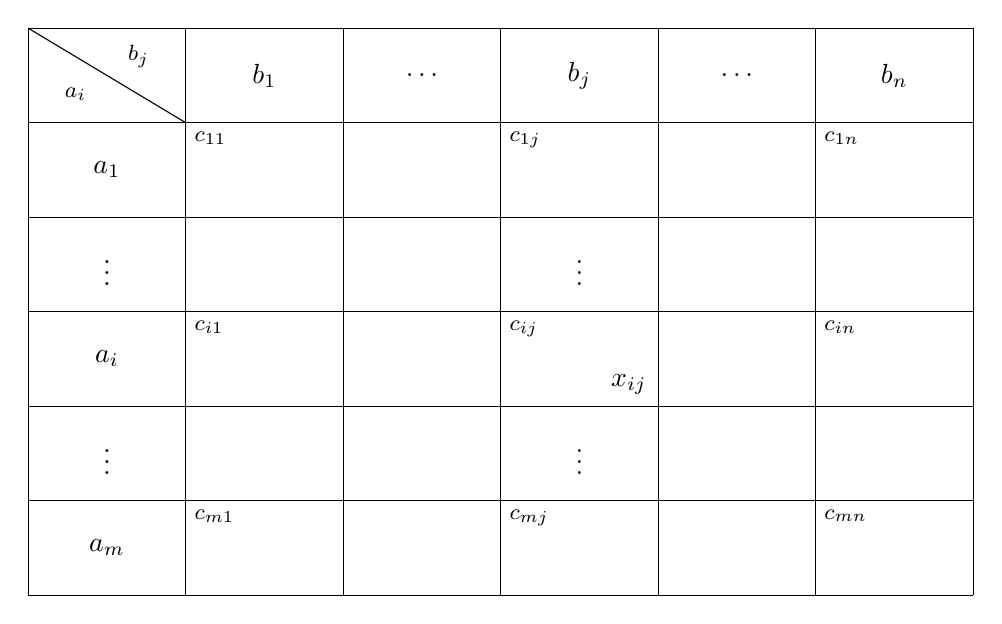
\begin{tikzpicture}[x=2cm, y=1.2cm]
        % Vẽ các đường ngang
        \foreach \y in {0, -1, -2, -3, -4, -5, -6} {
            \draw (0,\y) -- (6,\y);
        }
        % Vẽ các đường dọc
        \foreach \x in {0, 1, 2, 3, 4, 5, 6} {
            \draw (\x,0) -- (\x,-6);
        }
        
        % Ô góc trên bên trái
        \draw (0,0) -- (1,-1);
        \node at (0.3,-0.7) {\footnotesize $a_i$};
        \node at (0.7,-0.3) {\footnotesize $b_j$};
        
        % Tiêu đề cột
        \node at (1.5,-0.5) {$b_1$};
        \node at (2.5,-0.5) {$\dots$};
        \node at (3.5,-0.5) {$b_j$};
        \node at (4.5,-0.5) {$\dots$};
        \node at (5.5,-0.5) {$b_n$};
        
        % Tiêu đề hàng
        \node at (0.5,-1.5) {$a_1$};
        \node at (0.5,-2.5) {$\vdots$};
        \node at (0.5,-3.5) {$a_i$};
        \node at (0.5,-4.5) {$\vdots$};
        \node at (0.5,-5.5) {$a_m$};
        
        % C_ij values (top left corner of each cell)
        \node[anchor=north west, inner sep=3pt] at (1,-1) {\footnotesize $c_{11}$};
        \node[anchor=north west, inner sep=3pt] at (3,-1) {\footnotesize $c_{1j}$};
        \node[anchor=north west, inner sep=3pt] at (5,-1) {\footnotesize $c_{1n}$};
        
        \node at (3.5,-2.5) {$\vdots$};
        
        \node[anchor=north west, inner sep=3pt] at (1,-3) {\footnotesize $c_{i1}$};
        \node[anchor=north west, inner sep=3pt] at (3,-3) {\footnotesize $c_{ij}$};
        \node[anchor=north west, inner sep=3pt] at (5,-3) {\footnotesize $c_{in}$};
        
        % x_ij value (bottom right corner of cell i,j)
        \node[anchor=south east, inner sep=4pt] at (4,-4) {$x_{ij}$};
        
        \node at (3.5,-4.5) {$\vdots$};
        
        \node[anchor=north west, inner sep=3pt] at (1,-5) {\footnotesize $c_{m1}$};
        \node[anchor=north west, inner sep=3pt] at (3,-5) {\footnotesize $c_{mj}$};
        \node[anchor=north west, inner sep=3pt] at (5,-5) {\footnotesize $c_{mn}$};
        
    \end{tikzpicture}
\end{figure}
Tập các ô nằm trong bảng vận tải, được ký hiệu là:
\[ T = \{(i,j) \mid 1 \le i \le m, 1 \le j \le n\} \]
Tại mỗi ô $(i,j) \in T$, chi phí vận chuyển đơn vị $c_{ij}$ được đặt ở góc trên bên trái. Khi xây dựng một phương án phân bổ $X = (x_{ij})$, nếu lượng hàng luân chuyển $x_{ij} > 0$, nó sẽ được ghi nhận vào góc dưới bên phải của ô tương ứng.

Mỗi ô $(i,j)$ trong bảng vận tải có một sự tương ứng song ánh với véc-tơ cột trong ma trận hệ số $A$ của bài toán. Đối với một phương án $X$ bất kỳ, tập hợp các ô có chứa lượng hàng phân bổ thực tế được gọi là tập các \textit{ô cơ sở} (hay ô chọn), ký hiệu là:
\[ G(X) = \{(i,j) \in T \mid x_{ij} > 0\} \]
Những ô còn lại với $x_{ij} = 0$ được xem là các \textit{ô phi cơ sở} (ô loại).

Theo lý thuyết QHTT, một phương án cực biên không suy biến của bài toán vận tải cỡ $m \times n$ sẽ chứa chính xác $(m+n-1)$ ô cơ sở \cite{bachkim}.

\subsection{Chu trình}
Chu trình là một khái niệm cốt lõi giúp phân tích và tối ưu hóa bài toán vận tải thông qua việc đánh giá các sự thay đổi dọc theo một vòng khép kín.

\begin{definition}[Chu trình]
    Một tập hợp các ô trong bảng vận tải được liên kết với nhau theo một thứ tự nhất định sẽ tạo thành một \textit{chu trình} nếu chúng đồng thời đáp ứng ba tiêu chí:
    \begin{itemize}
        \item[i)] Bất kỳ hai ô nào đứng liền kề nhau trong dãy đều phải nằm chung trong một hàng hoặc một cột;
        \item[ii)] Không cho phép ba ô bất kỳ trong dãy cùng nằm trên cùng hàng hoặc cùng cột;
        \item[iii)] Chuỗi các điểm phải khép kín, tức là ô khởi đầu và ô kết thúc phải nằm trên cùng một hàng hoặc cùng một cột.
    \end{itemize}
\end{definition}

\begin{figure}[H]
    \centering
    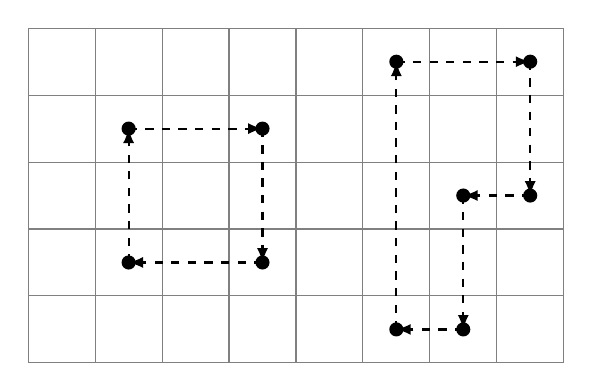
\begin{tikzpicture}[scale=0.85, every node/.style={scale=0.85}]
        % Khung lưới bảng vận tải
        \draw[step=1cm,color=gray] (0,0) grid (8,5);
        
        % Chu trình 1 (đơn giản 2x2)
        \fill (1.5, 3.5) circle (3pt);
        \fill (3.5, 3.5) circle (3pt);
        \fill (3.5, 1.5) circle (3pt);
        \fill (1.5, 1.5) circle (3pt);
        \draw[dashed, thick, -latex] (1.5, 3.5) -- (3.5, 3.5);
        \draw[dashed, thick, -latex] (3.5, 3.5) -- (3.5, 1.5);
        \draw[dashed, thick, -latex] (3.5, 1.5) -- (1.5, 1.5);
        \draw[dashed, thick, -latex] (1.5, 1.5) -- (1.5, 3.5);

        % Chu trình 2 (phức tạp hơn)
        \fill (5.5, 4.5) circle (3pt);
        \fill (7.5, 4.5) circle (3pt);
        \fill (7.5, 2.5) circle (3pt);
        \fill (6.5, 2.5) circle (3pt);
        \fill (6.5, 0.5) circle (3pt);
        \fill (5.5, 0.5) circle (3pt);
        
        \draw[dashed, thick, -latex] (5.5, 4.5) -- (7.5, 4.5);
        \draw[dashed, thick, -latex] (7.5, 4.5) -- (7.5, 2.5);
        \draw[dashed, thick, -latex] (7.5, 2.5) -- (6.5, 2.5);
        \draw[dashed, thick, -latex] (6.5, 2.5) -- (6.5, 0.5);
        \draw[dashed, thick, -latex] (6.5, 0.5) -- (5.5, 0.5);
        \draw[dashed, thick, -latex] (5.5, 0.5) -- (5.5, 4.5);
    \end{tikzpicture}
    \caption{Minh họa một số dạng chu trình trên bảng vận tải}
    \label{fig:cycle_examples}
\end{figure}

Từ góc độ đại số, chu trình có vai trò đặc biệt trong việc xác định tính độc lập tuyến tính của ma trận ràng buộc. Cụ thể, trong tài liệu \cite{bachkim}, ta đã có được hệ quả phục vụ cho việc xác định xem một phương án đã là phương án cực biên chưa:

\begin{corollary} \label{cor:basic_solution_cycle}
    Một phương án phân bổ $X = (x_{ij})$ đạt trạng thái cực biên khi và chỉ khi tập hợp các ô chứa hàng của nó, $G(X) = \{(i,j) \mid x_{ij} > 0\}$, không tạo thành bất kỳ chu trình nào.
\end{corollary}

Chính vì hệ quả này, trong thực hành giải bài toán vận tải, khái niệm phương án cực biên thường được gọi một cách nôm na là phương án không có chu trình.

\section{Các dạng bài toán vận tải cơ bản}

Trong báo cáo này, chúng ta sẽ tập trung vào những dạng bài toán vận tải căn bản nhất bao gồm bài toàn cân bằng thu phát và cách xử lý đối với trường hợp tổng lượng cung - cầu chênh lệch với nhau.

\subsection{Bài toán cân bằng thu phát}
Bài toán được gọi là cân bằng thu phát nếu tổng trữ lượng của các trạm phát bằng đúng tổng nhu cầu của các trạm thu:
\begin{equation} \label{eq:balanced}
    \sum_{i=1}^{m} a_i = \sum_{j=1}^{n} b_j
\end{equation}

Để chứng minh bài toán này luôn tồn tại phương án tối ưu, ta sẽ chứng minh tính đúng đắn của định lý sau:

\begin{theorem}[Định lý tồn tại] \label{thm:existence}
    Bài toán vận tải có phương án tối ưu khi và chỉ khi tổng tất cả các lượng phát bằng tổng tất cả các lượng thu, tức là
    \begin{equation}
        \sum_{i=1}^{m} a_i = \sum_{j=1}^{n} b_j \label{eq:balanced}
    \end{equation}
\end{theorem}
\begin{proof}

    \noindent ($\Rightarrow$) Giả sử bài toán vận tải có phương án tối ưu $x^* = (x_{ij}^*)$. Do đó $x^*$ phải thỏa mãn các ràng buộc, tức
    \[ \sum_{j=1}^{n} x_{ij}^* = a_i, \quad \forall i = \overline{1,m}  \quad \text{và} \quad \sum_{i=1}^{m} x_{ij}^* = b_j, \quad \forall j = \overline{1,n}. \]
    Và ta nhận được biểu thức \eqref{eq:balanced},
    \[ \sum_{i=1}^{m} a_i = \sum_{i=1}^{m} \sum_{j=1}^{n} x_{ij}^* = \sum_{j=1}^{n} \sum_{i=1}^{m} x_{ij}^* = \sum_{j=1}^{n} b_j. \]

    \noindent ($\Leftarrow$) Giả sử điều kiện \eqref{eq:balanced} thoả mãn, ta chứng minh bài toán vận tải có phương án tối ưu. Đặt
    \[ d = \sum_{i=1}^{m} a_i = \sum_{j=1}^{n} b_j \]
    và $\bar{x} = (\bar{x}_{ij})$, trong đó
    \[ \bar{x}_{ij} = \frac{a_i b_j}{d}, \quad \forall i = \overline{1,m}, \ \forall j = \overline{1,n}. \]

    Dễ thấy, $\bar{x}$ là một phương án chấp nhận được của bài toán vận tải, vậy nên tập chấp nhận được của bài toán khác rỗng.
    
    Do các ràng buộc cung cầu nên phương án chấp nhận được bất kỳ $x = (x_{ij})$ sao cho $x_{ij} \le \min\{a_i, b_j\}$ với mọi $i = \overline{1,m}, \ j = \overline{1,n}$. Vậy nên ta chứng minh được tập các phương án chấp nhận được là bị chặn. 
    
    Theo định lý cơ bản của QHTT (Định lý Weierstrass), một hàm mục tiêu liên tục trên một tập khác rỗng và bị chặn thì bài toán vận tải có phương án tối ưu và đạt tại ít nhất một phương án cực biên.
\end{proof}

Điều kiện \eqref{eq:balanced} được gọi là \textit{điều kiện cân bằng thu phát} và bài toán vận tải thoả mãn ràng buộc này gọi là \textit{bài toán vận tải cân bằng}. Từ đây trở đi, nếu không nói gì thêm thì bài toán vận tải được xét luôn thỏa mãn điều kiện cân bằng thu phát.

\subsection{Bài toán không cân bằng thu phát}
Trong thực tế, hiếm khi tổng lượng cung bằng đúng tổng lượng cầu. Khi đó, mô hình của bài toán sẽ chứa các bất phương trình thay vì phương trình. Để giải quyết, ta đưa các bất phương trình này về dạng phương trình bằng cách bổ sung các biến phụ, tương ứng với việc tạo ra các điểm thu giả hoặc điểm phát giả \cite{bachkim}.
    
\textbf{Trường hợp 1: Tổng cung lớn hơn tổng cầu}
\[ \sum_{i=1}^{m} a_i > \sum_{j=1}^{n} b_j \]
Lúc này, lượng hàng chở đi từ các trạm phát có thể nhỏ hơn trữ lượng $a_i$ nhưng tổng lượng hàng đến các trạm thu phải bằng đúng $b_j$. Hệ ràng buộc khi đó sẽ trở thành:
\begin{align*}
    \sum_{j=1}^{n} x_{ij} &\le a_i, \quad \forall i = 1, \dots, m \\
    \sum_{i=1}^{m} x_{ij} &= b_j, \quad \forall j = 1, \dots, n
\end{align*}
Để chuyển bất phương trình thành phương trình, ta đưa thêm vào mỗi ràng buộc hàng $i$ một biến phụ $x_{i, n+1} \ge 0$. Khi đó:
\begin{align*}
    \sum_{j=1}^{n} x_{ij} + x_{i, n+1} &= a_i, \quad \forall i = 1, \dots, m
\end{align*}
Lấy tổng tất cả các phương trình, ta tìm được tổng giá trị của các biến phụ:
\[ \sum_{i=1}^{m} x_{i, n+1} = \sum_{i=1}^{m} a_i - \sum_{j=1}^{n} b_j = b_{n+1} > 0 \]

Về mặt kinh tế, điều này tương đương với việc ta thêm một trạm thu giả, lượng hàng $x_{i, n+1}$ phân bổ vào trạm thu giả chính là lượng hàng tồn kho chưa được vận chuyển đi tại trạm phát $i$. Cước phí vận chuyển tới trạm giả được coi bằng không ($c_{i, n+1} = 0, \forall i$). Bài toán ban đầu trở thành bài toán cân bằng kích thước $m \times (n+1)$.
    
\textbf{Trường hợp 2: Tổng cung nhỏ hơn tổng cầu}
\[ \sum_{i=1}^{m} a_i < \sum_{j=1}^{n} b_j \]
Lúc này, toàn bộ hàng hóa đều được vận chuyển đi nhưng một số trạm thu sẽ không nhận đủ hàng. Hệ ràng buộc trở thành:
\begin{align*}
    \sum_{j=1}^{n} x_{ij} &= a_i, \quad \forall i = 1, \dots, m \\
    \sum_{i=1}^{m} x_{ij} &\le b_j, \quad \forall j = 1, \dots, n
\end{align*}

Tương tự với cách xử lý ở trên, ta thêm vào mỗi ràng buộc cột $j$ một biến phụ $x_{m+1, j} \ge 0$ để biến thành đẳng thức:
\begin{align*}
    \sum_{i=1}^{m} x_{ij} + x_{m+1, j} &= b_j, \quad \forall j = 1, \dots, n
\end{align*}
Tổng giá trị của các biến phụ lúc này là:
\[ \sum_{j=1}^{n} x_{m+1, j} = \sum_{j=1}^{n} b_j - \sum_{i=1}^{m} a_i = a_{m+1} > 0 \]

Ta vừa thêm một trạm phát giả thứ $m+1$ với trữ lượng ảo $a_{m+1} = \sum b_j - \sum a_i$. Biến $x_{m+1, j}$ đại diện cho lượng hàng bị thiếu hụt tại trạm thu $j$. Cước phí từ trạm phát giả tới mọi trạm thu được gán bằng không ($c_{m+1, j} = 0, \forall j$), trừ trường hợp có quy định về chi phí phạt do thiếu hàng (khi đó $c_{m+1, j} = M > 0$). Bài toán ban đầu trở thành bài toán cân bằng kích thước $(m+1) \times n$.

\vspace{0.5cm}
\begin{conclusion}
Bằng kỹ thuật thêm biến phụ, mọi bài toán vận tải mở đều có thể đưa được về bài toán vận tải cân bằng thu phát. Do đó, trong các nghiên cứu thuật toán tiếp theo, ta mặc định bài toán luôn thỏa mãn điều kiện $\sum a_i = \sum b_j$.
\end{conclusion}


\end{document}